%%%%%%%%%%%%%%%%%%%%%%%%%%%%%%%%%%%%%%%%%%%%%%%%%%%%%%%%%%%%%%%%%%%%%%%%%%%%%
%%
%% This file provides a template that can be used in concert with the
%% ohio-etd class to generate an electronic thesis or dissertation which
%% meets the formatting requirements at Ohio University.
%%
%% To use the template, copy this file (template.tex) and ohio-etd.cls into
%% the same directory and edit this template as required.  Reference
%% ohio-etd.pdf for additional instructions on using this class.
%%
%%%%%%%%%%%%%%%%%%%%%%%%%%%%%%%%%%%%%%%%%%%%%%%%%%%%%%%%%%%%%%%%%%%%%%%%%%%%%


%% Load the class.  Available options are: numbered, pdftex, cmfont,
%% singlespacetables, draft, 11pt, 12pt, leqno, and fleqn

\documentclass[numbered,pdftex]{ohio-etd}


%% Other packages that may be of use.  Delete or comment out (using a
%% percent sign in the first column) if they are not desired.  Reference
%% the corresponding documentation for more information on how to use these
%% packages.

\usepackage[square,sort&compress,numbers]{natbib} % Provides formatting for
                                                  % citations
\usepackage{textcomp} % Provides math symbols that can be used in text mode
\usepackage{amssymb}  % Provides additional AMS math symbols.  Note that
                      % amsmath is loaded as part of the ohio-etd class
\usepackage{bm}       % Provides bold-faced math symbols
\usepackage{booktabs} % Provides improved table formatting
\usepackage{dcolumn}  % Provides table columns aligned at decimal points
\usepackage{multirow} % Provides table elements spanning multiple rows
\usepackage{graphicx} % Standard package to incorporate graphics
\usepackage[printonlyused]{acronym} % Provides a method for incorporating
                                    % acronyms and building an acronym list

\graphicspath{{figures/}} % Allows graphics files to be stored in a
                          % separate directory



%% Required front matter definitions

\degree    {MS}              % MS, MA, MCTP, or PhD
\graduation{May}{2018}    % May, August, or December 

\title     {A Proposal for a Parameterized Circulating Vector Field Guidance for Fixed Wing Unmanned Aerial Vehicles}
\author    {Garrett S.}{Clem} 

\advisor   {Dr. Jay Wilhelm}{Assistant Professor}
\dean      {Dr. Dennis Irwin}{Dean of Students}

\program   {Mechanical Engineering}            % e.g. Electrical Engineering
\department{Department of Something} % e.g. School of Electrical Engineering 
                                     %      and Computer Science
\college   {Russ College of Engineering and Technology}   % e.g. Russ College of Engineering and
                                     %      Technology

\abstract  {Insert your abstract here}

%% Optional front matter definitions.  Delete or comment out if not needed

\coadvisor {Coadvisor's Full Name}{Coadvisor's Full Title}

\dedication{Insert your dedication here.\\ A double backslash can be used
  to force line breaks if desired.}

\acknowledgments{Insert your acknowledgments here or comment out this line.}
%% If you prefer to provide "acknowledgements" instead (note the added "e"
%% between the "g" and the "m") then add the "e" in the macro name so that
%% it reads "\acknowledgements".}

%% Additional "lists" can be added to the end of the front matter using the
%% \addlistof macro.  For example:
\addlistof{Symbols}{Insert your list of symbols here or comment out this line.}
%% Note that the command "\input{symbols}" can be used if the symbol list is
%% contained in a separate file called "symbols.tex"}

\addlistof{Acronyms}{Insert your list of acronyms here or comment out this line}
%% Use "\input{acronyms}" if the acronym list is in a separate file called
%% "acronyms.tex".  Note that the formatting generated by the acronym package
%% can be forced into singlespaced text by inserting "\setlength\itemsep{0pt}
%% \setlength\parskip{0pt}" into the "acronym" environment.} 

%% For documents created by government employees as part of their
%% employment.  The wording of the disclaimer can be specified using an
%% option.  See the documentation for more information.

% \govtdisclaimer    

% \notables  % Prevent a list of tables from being created
% \nofigures % Prevent a list of figures from being created

\begin{document}

\makefrontmatter    % Creates all of the front matter pages.

%% Body of the text follows, using \chapter, \section, \subsection,
%% \subsubsection, \paragraph, and \subparagraph to generate the
%% section headings.  For convenience, it may be useful to break the
%% full document into separate files, perhaps divided by chapters.  In
%% that case, the files would be loaded here using "\input{filename}"


%%%% -------- Points that I may want to include, but am not sure where yet --------%
%
% Its not uncommon for a simplified vehicle to be used (Dubins, simple constraints, etc)
% it is often assumed that there exists an autopilot that controls the heading and flight path angle and the system representing the uav is simplified to a dubins path
%
%	[Chen, Chang, Agate 2009]
%	[Liang, Jia 2017]
%	[Nelson, Barber, 2005]
%	[Griffiths 2006]
%	[Jung et al, 2016]
%	[]
%
% Vector Normalization
%	[Chen,Change, Agate 2009] (lambda)
%
%
% Ways to produce vector fields
%	Lyapunov
%	Intersection of surfaces [Goncalves]
%	Tangent Vector Field Guidance [Chen, Hang, Agate 2009]
%	Tangent Vector Field Guidance [Liang, Jia 2017]
%
%
%
%
% Vector field is an attractive guidance method for several reasons
% 	Account for wind disturbance
%	Vehicle will have continuous guidance
%	A single field can provide guidance for many initial conditions
%
%
%
% We desire to calculate the input u for the vehicle such that the UAV navigates to the goal while avoiding static obstacles
% in such a way to minimize the distance or time
%
%
%
%
% Clarification as to what a vector field is, what a potential field is, etc. Vector field is a space of n dimensions 
% that has an associated vector for each point in space. These vector fields can be constructed in a number of different 
% ways and it is useful to categorize them. In this literature potential fields will describe a vector field that is
% generated by langragian equations and by the principle of least action. Path following vector fields will be in reference
% to vector feilds that converge and follow a pre-defined path. (Then transistion into potential fields and VF discussion, how % they are made, what they are used for, the problems that we face when formulating them)
%
%
%
%%%% ---------------------------------------------------------------------------%

%Remove most references to multirotor technology, acknowledge its existience and move on


\chapter{Introduction}

Unmanned Aerial Vehicles (UAVs) can be used for a multitude of complex tasks such as surveillance, reconnaissance, aerial photography, delivery, and for defense. Accomplishing these tasks require robust and fast execution of three distinct subsystems consisting of navigation, guidance, and control. 
\section{Motivation and Problem Statement}

%UAVs commercially available, ease of use, inexpensive, open source community, wells supported

\section{Methods Overview}
\section{Phases}
\section{Summary of Objectives}
\begin{itemize}

\item Develop a parameterized circulation method that eliminates the singularity and guides a UAV around an obstacle and to a target. The parametrized circulation term $f(heading,closing velocity, position, turn rate)$ and would be determined by minimizing a cost.


\item Simulate and compare the parametrized circulation with a non parametrized VF guidance for circular and elliptical obstacles

\item Emulate fixed wing algorithm with a ground robot to validate simulation results and demonstrate real time VF guidance is achievable with parametrized circulation modification


\end{itemize}



\chapter{Literature Review}
\section{Literature Review Introduction}
 %==========================================================================================
% Tell the reader what you're going to tell them
% - Fixed wing operation
% - Navigation
% - Guidance and control
% - Obstacle avoidance and circumnavigation by time paramerterized vector field
% 
% Tell the reader something
% Tell them what you told them


\section{Unmanned Aerial Vehicles}

In literature, UAVs generally occupy one of two categories consisting of fixed wing aircraft and multi-rotor aircraft. Fixed wing aircraft can carry a large payload and are ideal for long endurance missions, whereas multi-rotor aircraft are used when hovering or high maneuverability is desired. Both categories of vehicles require navigation, guidance, and control to maintain flight and accomplish their task. These processes are often automated and programmed into flight controllers that are placed on-board the aircraft itself. 

 - Miniature Aerial Vehicles (Classification, what makes them different then traditional fixed wing UAVs...etc)

 - Tasks (path following, waypoint navigation, loitering)
 - Trajectory following versus path following. Trajectory following is not as popular for MAVs since the added constraint is more difficult to achieve compared to path following
 
 - The autopilots that operate the UAVs do so through several layers of systems known as navigation, guidance, and control NGL
 
 - Path planning
 - Guidance
 - Control
 
 - Who (Civilians and military)
 - Military uses for surveillance, reconnaissance, data transmission
 - Civilians have found uses such as aerial photography, environmental monitoring, and racing, fire monitoring
 
 - One of the many strengths in unmanned systems is the potential for autonomy (equivalent to fire-and-forget). Autonomy frees up operators for other decision making
 
 \begin{equation}\label{dubinsx}
 \dot{x} = V\cos(\theta)
 \end{equation}
  \begin{equation}\label{dubinsy}
 \dot{y} = V\sin(\theta)
 \end{equation}
 


\subsection{Flight Mechanics}

- Lift
- Thrust
- Drag

\begin{figure}[h]
	\centering
	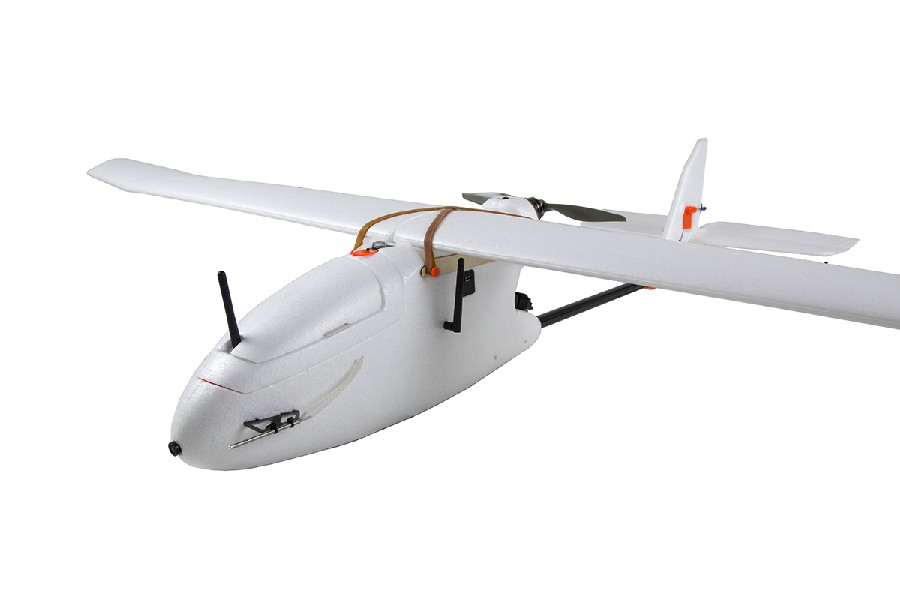
\includegraphics[width=0.7\linewidth]{PaperFigures/fixedwing}
	\caption{Fixed Wing UAV}
	\label{fig:fixedwing}
\end{figure}



- Forward velocity constraints, turn rate constraints \\
- Transition could be the autopilot ensures that the vehicle does not violate these constraints or attempt to \\
- Autopilot (combination of hardware and software, takes mission objectives and produces necessary actuator output)

% "After planning waypoints, paths are then planned by connecting points together" [Jung et al 2016]
% - These are connected a number of ways, go to jung et al for more information. Dubins, etc
% - After paths are generated, guidance takes over to guide UAV to converge and stay on the path
%



\begin{figure}[h]
	\centering
	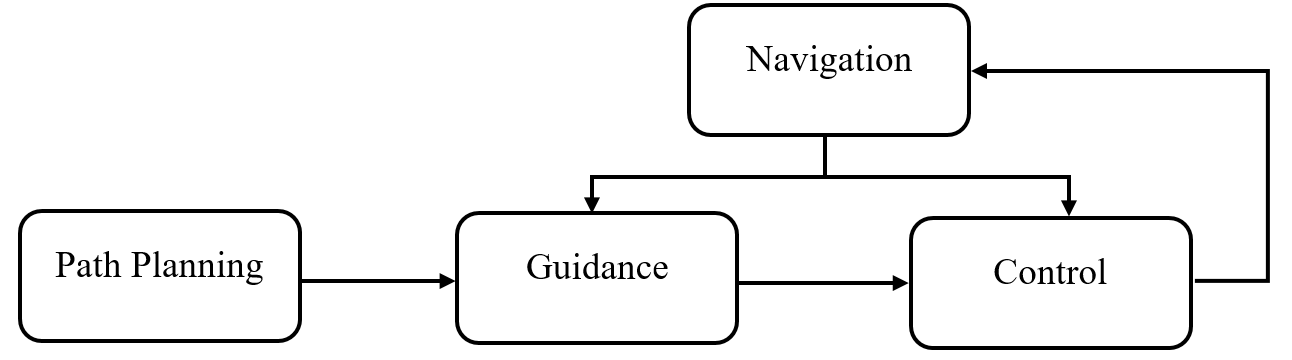
\includegraphics[width=0.7\linewidth]{PaperFigures/ngcFlow}
	\caption{Navigation Guidance and Control Flowchart}
	\label{fig:ngcflow}
\end{figure}



\section{Navigation}
Before commanding a vehicle to a given task it is paramount that the location of a vehicle with respect to some reference point is known. Measuring, filtering, and estimating the location of a vehicle generally falls under the study of navigation. Commanding a vehicles heading and general operation is provided by a guidance system. Maintaining vehicle stability and reducing any errors is the responsibility of a control system. 

Sensor packages containing GPS receivers, barometers, and compasses measure the location and heading of a vehicle. Data is always subject to uncertainty caused by process and measurement noise. Filtering measurements with Kalman filters produce estimates that more accurately represent the location and heading.



\section{Guidance and Control}

%===============
%
% Depending on the source, potential field may be referred to as a vector field, but for organizational purposes potential field will be classified separately as a potential gradient and vector field as a path converging and %  	following method
%
% Vector fields may be referred to as a potential field, but for organizational purposes they will be discussed as seperate methods all together where a potential field represents a potential gradient. A vector field represents a space of vectors whose integral lines converge and follow a path
%
Traditional guidance and control are considered separate and independent systems that only exchange the most basic information. High level guidance provides the control system with a commanded heading and velocity to guide the UAV to a path or waypoint designed by the path planner. Low level control accepts the guidance and attempts to drive the state error to zero while maintaining vehicle stability. As more complicated tasks are assigned to UAVs, such as converge and follow a moving path \cite{oliveira_moving_2016} either the guidance or control will become more complicated. The line between guidance and control is starting to become less tangible as the responsibilities of the guidance system becomes more intertwined with control systems. 

One notable field of study in robotic guidance is that of vector fields. Each point in the operational space of the robot is assigned a vector of \textit{n}-dimensions that can represent velocity, acceleration, or any arbitrary state. Vector fields have been shown to be an effective way to guide a UAV to a path and does so with less error and control effort than non-linear guidance, linear quadratic regulator, carrot chasing, and pure pursuit line of sight methods \cite{sujit_unmanned_2014}. There are many ways to build a vector field including potential Lagrangian functions \cite{khatib_real-time_1986}, Lyapunov navigation functions \cite{esposito_method_2002}\cite{frew_lyapunov_nodate} \cite{nelson_cooperative_2005}, and integral curves by intersection of surfaces \cite{goncalves_artificial_2009} \cite{goncalves_vector_2010}.


\subsection{Potential Field}
Potential field is a real-time robotic manipulator algorithm that distributes the task of goal seeking and obstacle avoidance among multiple layers of control \cite{khatib_real-time_1986}. The robot's workspace is represented as a gradient potential of attractive and repulsive artificial forces that drive the robot to a desired state. Goals are represented as an attractive force while obstacles provide a repulsive force. The potential field is constructed by modeling the robots motion in terms of Lagrangian mechanics shown in Equation \ref{LeeMotion}. The Lagrangian is defined as the difference in kinetic energy $T(x,\dot{x})$ and potential energy $U(x)$ in a system. The goal of the system imparts a potential $U_{xd}$ while obstacles impart a repulsive potential $U_o$. 

\begin{equation}\label{LeeMotion}
\frac{d}{dt} \left(\frac{\partial L}{\partial \dot{x}}\right) - \frac{\partial L}{\partial x} = F
\end{equation}

\begin{equation}\label{lagrange}
L(x,\dot{x}) = T(x,\dot{x}) - U(x)
\end{equation}

\begin{equation}\label{potential}
U_{art}(x) = U_{xd} + U_o(x)
\end{equation}

Potential field has been shown to be successful at driving a robot from an initial state to a goal state while avoiding obstacles by taking the path of least action formed by the gradient. One of the weaknesses of potential field identified early on is the methods susceptibility to local minima, preventing the robot from reaching the desired global minima, or goal state \cite{koren_potential_1991}. Local minima can be avoided in the potential field method if navigation functions are used \cite{goerzen_survey_2010}.\\

Potential field is useful for point-to-point guidance and control which is often the task of UAVs traveling to waypoints, however it is often desired for a UAV to converge to and follow a path. 

%%%%%%%%%% Additional points and clarification needed here before moving on
%
% Address navigation functions
% Re-read Goerzens review article and understand the scope of PF to a better degree
% Improve the transition to vector field
%		- Potential fields have proven to be useful for point-to-point navigation, however lack the framework for one of the common applications for fixed wing UAVs, path following
%
%

\subsection{Vector Field}

%Description into what the vector field actually is
% Vector field provides a directional guidance. Building that field can be done in a number of ways
%
% In cases referenced as lyapunov, the method is used to derive the vector field and prove stability
%
% Takes current vehicle position and guides UAV to the path
%
%
% Think about discussing the general behavior of vector field paths (When far away from the path, the vector tends to point more perpendicular, as you approach the path, it transitions to trangent to the path)
% 

Several methods have been developed to generate vector fields that converge to and follow paths. Histogram virtual force field (VFF) breaks the workspace into discrete cells that contain information in regards to the certainty of the presence of an obstacle \cite{borenstein_real-time_1990} \cite{borenstein_vector_1991}. Cells containing an obstacle apply an artificial guidance force away from the cell. Goals apply a global attractive force that drive the robot towards the desired state. The resultant guidance vector for the VFF method is the sum of the contributions of obstacle repulsive cells and the globally attractive goal. Lyapunov and navigation functions have been successfully used to provide guidance for converging to and following a path. Nelson et al. developed a method for generating a vector field that converges to and follows a path for line and circular primitives \cite{nelson_cooperative_2005}. Sinks, dead zones, and singularities were avoided when constructing more complex flight paths from the primitives by only allowing a single field to be active at any time. A vector field construction method for curved paths was presented in \cite{griffiths_vector_2006} by extending Nelson's method. Elliptical paths have been generated by from primitives by applying coordinate transformations to the field \cite{frew_lyapunov_nodate}.




Vector fields have many advantages to traditional guidance. UAVs often encounter disturbances in the form of wind which can be difficult to plan for. In the event a UAV encounters wind disturbances and is pushed off course, the field will drive the vehicle back on course \cite{de_marina_guidance_2017}. In addition to path following, vector field has been used to track a moving target in 3D \cite{miao_orthogonal_2016}. When the location of the target is unknown, loitering about an uncertain target can be achieved by building a circular vector field and applying a linear coordinate transformation to form an elliptical loiter based on the uncertainty in targets position estimate \cite{frew_cooperative_2007}. 


%
% 3D Vector field 
% \cite{meenakshisundaram_vector_2010}
%
%
%

- Following curved paths in a constant wind \cite{griffiths_vector_2006}


%%%%%% Points to make for vector field
%
% - Disturbance rejection (wind)
% - Well suited for unplanned obstacle avoidance
% - Many applications are best described as path following instead of singular point convergence like potential field
% - Standoff tracking of uncertain targets
%
%

Another method for constructing a vector field is by forming integral curves that converge at the intersection of surfaces \cite{goncalves_artificial_2009}. 

- construct an n-dimensional vector field by forming integral curves that converge at the intersection of surfaces
- Field is a result of the sum of 3 terms
  - Convergence
  - Circulation
  - Time varying\\


% Note, modify the field equation to what jay has in his paper
\begin{equation}\label{gonFieldeq}
\boldsymbol{u} = G\nabla_qV+H\wedge_{i=1}\nabla_q\alpha_i - M(\alpha)^{-1}\boldsymbol{a}(\alpha)
\end{equation}

- Define all variables
	- u is the resulting 2x1 vector
	- Gradient
	- $alpha_i$ is a surface function
	- Wedge product simplifies to cross product in 2d
	- G, H, L scalar weighting quantities 
	- The intersection of the surfaces represents a path to converge and follow
	- Cylinder and plane example


\begin{figure}[h]
	\centering
	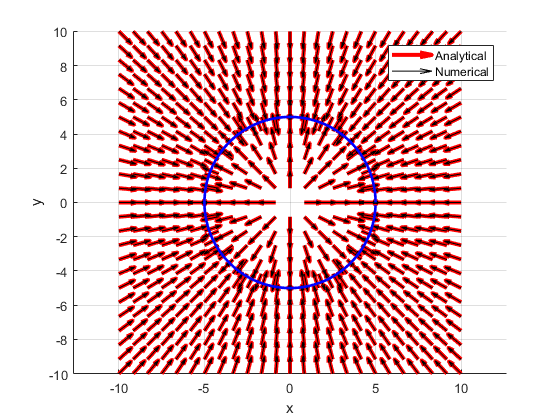
\includegraphics[width=0.7\linewidth]{PaperFigures/convergence}
	\caption{}
	\label{fig:convergence}
	
\end{figure}

\begin{figure}[h]
	\centering
	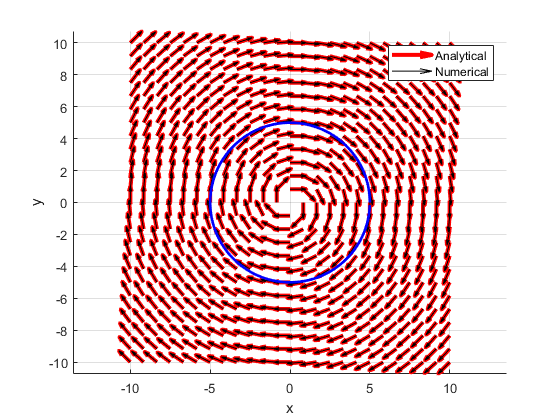
\includegraphics[width=0.7\linewidth]{PaperFigures/circulation}
	\caption{}
	\label{fig:circulation}
\end{figure}

\begin{figure}[h]
	\centering
	\includegraphics[width=0.7\linewidth]{"PaperFigures/time varying"}
	\caption{}
	\label{fig:time-varying}
\end{figure}


\begin{figure}[h]
	\centering
	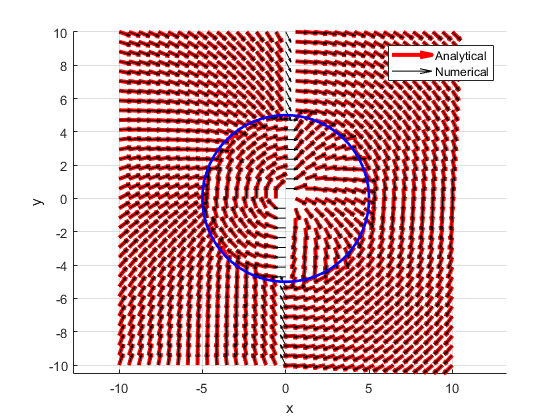
\includegraphics[width=0.7\linewidth]{PaperFigures/total}
	\caption{}
	\label{fig:total}
\end{figure}

\begin{itemize}
	\item Cooperative Standoff Tracking of Uncertain moving targets (2007, Frew)
	\item VF usefulness extended to loitering about an uncertain target
	\item Lyapunov vector field generation for a circular loiter
	\item Linear transformation applied to stretch the field into an ellipse shape
\end{itemize}




\section{Simulation and Emulation}
- As new features and improvements are made to the autopilot software, it is often useful to test the performance of the software in a virtual environment. The process of simulating the autopilot software is called Software in the Loop (SITL).

An additional testbed for new navigation, guidance, and control algorithms is the method of emulation. Emulation is the process of mimicking the kinematics of a complex dynamic system on a simplified system. Fixed wing UAV emulation has been observed in \cite{louali_designing_2014}, \cite{ren_experimental_2007}, and \cite{louali_experimental_2016}.

%Many simplifications are made when developing a simulation model, which may fail to capture some of the complexities of real world systems. Emulation provides another tool for testing an algorithm prior to putting it on actual flight hardware to validate, diagnose, and debug the proposed NGL systems. [Beard, Mclain,book]

\section{Literature Review Summary}


\chapter{Methodology}






























%- Hardware and software packages \\
%- Collect and filter sensor data \\
%- Receive mission commands (Go-to, Loiter, Hover) \\
%- Transmit mission critical information to ground station \\
%- Execute missions and maintain vehicle stability \\
%
%- Many autopilots are available \\
%- PX4 is an open-source autopilot software that can be ran on a number of hardware platforms including the Pixhawk, PixRacer, Parrot Bebop, and Crazyflie. Integrating the pixhawk firmware into a companion computer is useful because more complex software can be ran on-board as well as multiple computer languages. \\
%
%
%
%\subsection{Simulation}
%- As new features and improvements are made to the autopilot software, it is often useful to test the performance of the software in a virtual environment. The process of simulating the autopilot software is called Software in the Loop (SITL).
%
%\subsection{Emulation}
%
%An additional testbed for new navigation, guidance, and control algorithms is the method of emulation. Emulation is the process of mimicking the kinematics of a complex dynamic system on a simplified system. Fixed wing UAV emulation has been observed in \cite{louali_designing_2014}, \cite{ren_experimental_2007}, and \cite{louali_experimental_2016}.
%
%\section{Path Planning}
%\begin{itemize}
%
%%In no particular order of importance, all points that should be discussed
%\item Current state to goal state while passing through objectives
%\item High level obstacle avoidance
%\item Line or series of waypoints
%\item How vehicle reaches line or points not necessarily considered
%\item Responsibility of guidance
%\item Avoid collisions, seeking goals
%\end{itemize}
%
%\section{Guidance}
%\subsection{Potential Field}
%\begin{itemize}
%\item Potential field (what is it) (edge of bowl, marble, goal, obstacles)
%\item Calculation time
%\begin{itemize}
%\item Long time to calculate
%\item Environment changes, entire field has to be regenerated
%\item Improvements could be made with better computing methods . . .
%\end{itemize}
%
%\item Local minimums
%\begin{itemize}
%\item Local minimums are a significant area of study in potential field
%\item Examples of how the problem is being addressed
%\item Common issue across the board - No clear solution in sight
%\item As missions become more complex, the problem only worsens
%\end{itemize}
%
%\end{itemize}
%
%\subsection{Vector Field}
%\begin{itemize}
%\item First appearance of vector field (Histogram approach) [Koren 1989] (read before typing it out)
%
%\item Experiments with sonar sensor robots [Koren and B 1991]
%
%\item \citep{borenstein_real-time_1990} Improvements on previous vector field histogram
%\item Ground robot
%\item Later work provided improvements
%\item Limitations, size of cells, instability and oscillations
%\item Problems with VF, used as a general path planner with another local path planner on top 
%\item (transition)
%
%
%\item First instance of generating a field for converging onto paths made of straight line and circular segments (Nelson, Barber, 2006)
%\item Field construction of Nelson and Barber (More reading)
%\item Added benefit of VF is adding component to counteract wind
%
%\item Cooperative Standoff Tracking of Uncertain moving targets (2007, Frew)
%\item VF usefulness extended to loitering about an uncertain target
%\item Lyapunov vector field generation for a circular loiter
%\item Linear transformation applied to stretch the field into an ellipse shape
%\end{itemize}
%
%\subsection{Literature Review Summary}
%
%
%\chapter{Methodology}

%===****====
% Remember to include something about latency and control delay. Adding a look-ahead functionality may improve the performance of the VF guidance


%% The \references command marks the point where the bibliography will
%% be inserted.  In the example below, the BibTeX commands are
%% inserted into the macro definition, but one could also manually
%% enter the bibliography entries if desired.
\references{
  %ETD does not define a particular required bibliography style.
  %They DO require entries to end in a period UNLESS they end in a URL
  %or DOI AND that DOIs be set in the same font as everything else.
  %I have modified the alphaurl style file, to conform to these requirements.
  \bibliographystyle{alphaurl_etd}   
  \bibliography{bib}
}

\appendix           % Indicates the transition from chapters to appendices.  
                    % Subsequent 

\chapter{An Appendix}
\section{A Section in the Appendix}

\end{document}
